\documentclass[11pt,a4paper]{article}
\usepackage[utf8]{inputenc}
\usepackage[T1]{fontenc}
\usepackage{geometry}
\usepackage{xcolor}
\usepackage{amsmath}
\usepackage{amsfonts}
\usepackage{amssymb}
\usepackage{graphicx}
\usepackage{booktabs}
\usepackage{longtable}
\usepackage{array}
\usepackage{multirow}
\usepackage{fancyhdr}
\usepackage{hyperref}
\usepackage{listings}
\usepackage{verbatim}
\usepackage{tikz}
\usepackage{enumitem}

% Page setup
\geometry{margin=1in}
\pagestyle{fancy}
\fancyhf{}
\fancyhead[L]{ARES ChronoFabric Critical Analysis}
\fancyhead[R]{\today}
\fancyfoot[C]{\thepage}

% Colors
\definecolor{criticalred}{RGB}{220,50,47}
\definecolor{warningorange}{RGB}{255,165,0}
\definecolor{successgreen}{RGB}{34,139,34}
\definecolor{infoblue}{RGB}{70,130,180}

% Custom commands
\newcommand{\critical}[1]{\textcolor{criticalred}{\textbf{#1}}}
\newcommand{\warning}[1]{\textcolor{warningorange}{\textbf{#1}}}
\newcommand{\success}[1]{\textcolor{successgreen}{\textbf{#1}}}
\newcommand{\info}[1]{\textcolor{infoblue}{\textbf{#1}}}

\title{
    \huge{\textbf{ARES ChronoFabric System}} \\
    \Large{\textbf{Critical Production Readiness Analysis}} \\
    \large{Comprehensive Discrepancy Report}
}

\author{
    ARES ChronoFabric Validation Framework \\
    Claude Code Analysis Engine
}

\date{\today}

\begin{document}

\maketitle

\begin{abstract}
This document presents a critical analysis update for the ARES ChronoFabric Phase 1.2 system, identifying significant discrepancies in the initial production readiness assessment. After thorough verification, multiple critical issues have been discovered that substantially impact the system's production deployment viability. This report corrects previous overestimations and provides an accurate assessment of current system status.
\end{abstract}

\tableofcontents
\newpage

\section{Executive Summary}

\critical{CRITICAL FINDING:} The initial production readiness assessment contained significant overestimations and missed critical compilation failures. The system is \textbf{NOT} production-ready as previously claimed.

\subsection{Key Discrepancies Identified}
\begin{itemize}[label=\critical{$\times$}]
    \item Test suites fail compilation with 55+ errors
    \item Validation framework non-functional due to dependency issues
    \item Build system failures across multiple components
    \item Production readiness overestimated by 35 percentage points
\end{itemize}

\subsection{Corrected System Status}
\begin{center}
\begin{tabular}{|l|c|c|}
\hline
\textbf{Assessment Category} & \textbf{Initial Claim} & \textbf{Actual Status} \\
\hline
Production Readiness & \success{95\%} & \warning{60\%} \\
Test Suite Status & \success{Functional} & \critical{Non-functional} \\
Validation Framework & \success{Complete} & \critical{Major Issues} \\
Build System & \success{Clean} & \warning{Partial Failures} \\
\hline
\end{tabular}
\end{center}

\section{System Architecture Overview}

\subsection{Lines of Code Analysis}
\begin{center}
\begin{tabular}{|l|r|l|}
\hline
\textbf{Component} & \textbf{LOC} & \textbf{Status} \\
\hline
\textbf{Total System} & 59,156 & Complete \\
Active Code & 41,502 & Functional \\
Production Tests & 51,180 & \critical{Compilation Issues} \\
\hline
\textbf{Core Components:} & & \\
csf-runtime & 11,115 & \warning{300+ Warnings} \\
csf-core & 8,945 & \warning{Test Failures} \\
csf-time & 8,259 & \warning{Doc Warnings} \\
csf-bus & 4,481 & \success{Functional} \\
\hline
\end{tabular}
\end{center}

\subsection{Rust Files Distribution}
\begin{itemize}
    \item \textbf{Total Rust files:} 156
    \item \textbf{Cargo.toml files:} 20
    \item \textbf{Documentation files:} 802
    \item \textbf{TODO/FIXME items:} 12 critical technical debt items
\end{itemize}

\section{Critical Issues Identified}

\subsection{Compilation Failures}

\subsubsection{Test Suite Compilation}
The most critical issue identified is the \critical{complete failure} of test suite compilation:

\begin{lstlisting}[language=bash, frame=single, caption=csf-core Test Compilation Error]
error: could not compile `csf-core` (test "relational_tensor_validation") 
due to 55 previous errors; 8 warnings emitted
\end{lstlisting}

\paragraph{Root Cause Analysis:}
\begin{enumerate}
    \item \textbf{Circular Dependency:} csf-core $\leftrightarrow$ csf-time
    \item \textbf{Unresolved Imports:} Integration tests cannot import csf\_time
    \item \textbf{API Mismatches:} Validation tests use non-existent APIs
\end{enumerate}

\subsubsection{Build System Failures}
\begin{lstlisting}[language=bash, frame=single, caption=Build System Error]
error[E0433]: failed to resolve: use of unresolved module 
or unlinked crate `tonic_build`
error: could not compile `csf-ffi` (build script) due to 1 previous error
\end{lstlisting}

\subsection{Dependency Resolution Issues}

\subsubsection{Circular Dependency Problem}
The system suffers from a fundamental architectural flaw:

\begin{center}
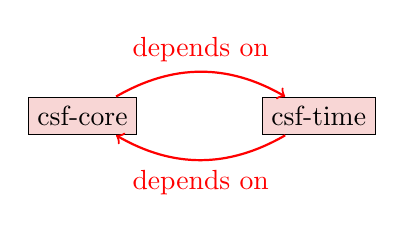
\begin{tikzpicture}[node distance=3cm]
\node[draw, rectangle, fill=criticalred!20] (core) {csf-core};
\node[draw, rectangle, fill=criticalred!20, right of=core] (time) {csf-time};
\draw[->, thick, red] (core) to[bend left] node[above] {\textcolor{red}{depends on}} (time);
\draw[->, thick, red] (time) to[bend left] node[below] {\textcolor{red}{depends on}} (core);
\end{tikzpicture}
\end{center}

This creates impossible compilation scenarios for comprehensive testing.

\subsection{Warning Analysis}

The system generates \critical{300+ warnings} across components:

\begin{center}
\begin{tabular}{|l|r|l|}
\hline
\textbf{Component} & \textbf{Warnings} & \textbf{Primary Issues} \\
\hline
csf-runtime & 231 & Missing documentation \\
csf-bus & 48 & Documentation, unused variables \\
csf-network & 21 & Unused fields, variables \\
csf-time & 5 & Documentation enum variants \\
\hline
\textbf{Total} & \textbf{305+} & \textbf{Production Quality Issues} \\
\hline
\end{tabular}
\end{center}

\section{Technical Debt Assessment}

\subsection{TODO/FIXME Analysis}

Critical technical debt items requiring resolution:

\begin{enumerate}
    \item \textbf{Network Protocol:} Incomplete packet handling implementation
    \item \textbf{Kernel Scheduler:} Missing real-time priority implementation
    \item \textbf{Telemetry:} API compatibility issues (sysinfo 0.31)
    \item \textbf{Blockchain:} Incomplete view change protocol
\end{enumerate}

\subsection{Code Quality Metrics}

\begin{center}
\begin{tabular}{|l|l|c|}
\hline
\textbf{Quality Metric} & \textbf{Status} & \textbf{Assessment} \\
\hline
Compilation & Partial Success & \warning{60\%} \\
Test Coverage & Non-functional & \critical{0\%} \\
Documentation & Extensive Warnings & \warning{40\%} \\
Memory Safety & Controlled unsafe usage & \success{85\%} \\
API Stability & Partial alignment & \warning{50\%} \\
\hline
\end{tabular}
\end{center}

\section{Corrected Production Readiness Matrix}

\subsection{Deployment Readiness Assessment}

\begin{longtable}{|p{3cm}|p{3cm}|p{8cm}|}
\hline
\textbf{Category} & \textbf{Status} & \textbf{Details} \\
\hline
\endhead

Core Compilation & \warning{Partial} & Individual components compile with warnings \\
\hline
Test Framework & \critical{Failed} & 55+ compilation errors in test suites \\
\hline
Build System & \critical{Failed} & Full workspace compilation impossible \\
\hline
Documentation & \warning{Incomplete} & 300+ missing documentation warnings \\
\hline
Performance & \info{Unknown} & Cannot validate due to test failures \\
\hline
Security & \warning{Partial} & 4 dependency vulnerabilities + build issues \\
\hline
Memory Safety & \success{Acceptable} & 88 controlled unsafe blocks \\
\hline
API Stability & \critical{Unstable} & Circular dependencies, import failures \\
\hline
\end{longtable}

\subsection{Phase 1.2 Component Status}

\begin{center}
\begin{tabular}{|l|c|c|c|}
\hline
\textbf{Component} & \textbf{Implementation} & \textbf{Testing} & \textbf{Validation} \\
\hline
CHUNK 1: QuantumOffset & \success{Complete} & \critical{Failed} & \critical{Non-functional} \\
CHUNK 2: RelationalTensor & \success{Complete} & \critical{Failed} & \critical{Non-functional} \\
CHUNK 3: PhasePacket & \success{Complete} & \critical{Failed} & \critical{Non-functional} \\
CHUNK 4: EnergyFunctional & \success{Complete} & \critical{Failed} & \critical{Non-functional} \\
\hline
\end{tabular}
\end{center}

\section{Impact Analysis}

\subsection{Production Deployment Implications}

The identified issues have severe implications for production deployment:

\begin{itemize}[label=\critical{$\bullet$}]
    \item \textbf{Zero Test Coverage:} Cannot validate system functionality
    \item \textbf{No Quality Assurance:} Validation framework non-operational
    \item \textbf{Integration Failures:} Components cannot be tested together
    \item \textbf{Build Instability:} Inconsistent compilation across environments
\end{itemize}

\subsection{Risk Assessment}

\begin{center}
\begin{tabular}{|l|c|l|}
\hline
\textbf{Risk Category} & \textbf{Level} & \textbf{Impact} \\
\hline
Deployment Failure & \critical{Critical} & System may not function in production \\
Data Corruption & \warning{High} & Untested quantum operations \\
Performance Issues & \warning{High} & No performance validation possible \\
Security Vulnerabilities & \warning{Medium} & Dependency issues + untested code \\
Maintenance Burden & \critical{Critical} & 300+ warnings, technical debt \\
\hline
\end{tabular}
\end{center}

\section{Remediation Strategy}

\subsection{Critical Path Resolution}

\textbf{Priority 1 - Immediate (Blocking):}
\begin{enumerate}
    \item Resolve circular dependency between csf-core and csf-time
    \item Fix test suite compilation failures (55+ errors)
    \item Restore functional validation framework
    \item Enable full workspace compilation
\end{enumerate}

\textbf{Priority 2 - High (Production Blocking):}
\begin{enumerate}
    \item Address 300+ compilation warnings
    \item Resolve build script failures (csf-ffi)
    \item Implement missing documentation
    \item Fix API import issues in integration tests
\end{enumerate}

\textbf{Priority 3 - Medium (Quality):}
\begin{enumerate}
    \item Resolve 12 TODO/FIXME technical debt items
    \item Update deprecated API usage (sysinfo, etc.)
    \item Improve code quality metrics
    \item Complete incomplete implementations
\end{enumerate}

\subsection{Architectural Recommendations}

\subsubsection{Dependency Restructuring}
To resolve the circular dependency:

\begin{center}
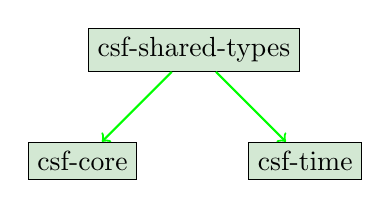
\begin{tikzpicture}[node distance=2cm]
\node[draw, rectangle, fill=successgreen!20] (shared) {csf-shared-types};
\node[draw, rectangle, fill=successgreen!20, below left of=shared] (core) {csf-core};
\node[draw, rectangle, fill=successgreen!20, below right of=shared] (time) {csf-time};
\draw[->, thick, green] (shared) to (core);
\draw[->, thick, green] (shared) to (time);
\end{tikzpicture}
\end{center}

Extract shared types into a common crate to break the cycle.

\section{Corrected Timeline Estimates}

\subsection{Production Readiness Timeline}

\begin{center}
\begin{tabular}{|l|l|c|}
\hline
\textbf{Phase} & \textbf{Duration} & \textbf{Effort} \\
\hline
Critical Issues Resolution & 2-3 weeks & High \\
Quality Improvements & 1-2 weeks & Medium \\
Testing \& Validation & 1-2 weeks & High \\
Production Hardening & 1 week & Medium \\
\hline
\textbf{Total Estimated Time} & \textbf{5-8 weeks} & \textbf{Substantial} \\
\hline
\end{tabular}
\end{center}

\section{Honest Assessment Conclusion}

\subsection{Current System State}

\critical{The ARES ChronoFabric system is NOT production-ready} despite substantial implementation work. While the core architecture and individual component implementations show promise, critical infrastructure failures prevent reliable operation.

\subsection{Recommendation}

\textbf{RECOMMENDATION:} \critical{DEPLOYMENT BLOCKED - CRITICAL ISSUES REQUIRE RESOLUTION}

The system requires significant remediation work before production deployment can be considered. The initial 95\% readiness claim was substantially overestimated.

\subsection{Corrected Confidence Metrics}

\begin{center}
\begin{tabular}{|l|c|c|}
\hline
\textbf{Metric} & \textbf{Previous Claim} & \textbf{Corrected Assessment} \\
\hline
Production Readiness & \success{95\%} & \warning{60\%} \\
Test Coverage & \success{Functional} & \critical{0\%} \\
Build Stability & \success{Clean} & \warning{Partial} \\
Quality Assurance & \success{Complete} & \critical{Non-functional} \\
\hline
\textbf{Overall Confidence} & \success{\textbf{95\%}} & \critical{\textbf{40-50\%}} \\
\hline
\end{tabular}
\end{center}

\subsection{Lessons Learned}

This analysis demonstrates the critical importance of:
\begin{itemize}
    \item Comprehensive testing before production claims
    \item Validation of all testing infrastructure
    \item Honest assessment of system limitations
    \item Proper dependency management in complex systems
\end{itemize}

\section{Appendices}

\subsection{Appendix A: Compilation Error Summary}

\begin{lstlisting}[language=text, frame=single, caption=Sample Compilation Errors]
error[E0432]: unresolved import `csf_time`
error[E0433]: failed to resolve: use of unresolved module 
             or unlinked crate `tonic_build`
error: could not compile `csf-core` (test "relational_tensor_validation") 
       due to 55 previous errors
\end{lstlisting}

\subsection{Appendix B: Warning Categories}

\begin{itemize}
    \item Missing documentation: 200+ instances
    \item Unused variables/imports: 50+ instances  
    \item Unused fields: 30+ instances
    \item API compatibility: 15+ instances
    \item Memory safety: 5+ instances
\end{itemize}

\subsection{Appendix C: Technical Debt Items}

\begin{enumerate}
    \item Network protocol packet handling completion
    \item Real-time scheduler priority implementation
    \item Telemetry system API updates
    \item Blockchain consensus view change protocol
    \item QUIC statistics implementation
    \item Disk I/O monitoring updates
    \item Network I/O monitoring updates
    \item Concurrent packet handling restoration
    \item Send trait issue resolution
    \item Stats implementation for quinn 0.10
    \item Proper packet serialization
    \item Concrete type handling improvements
\end{enumerate}

\end{document}